\chapter{L'Attività di Stage}
\label{3.0}
\thispagestyle{fancy} 

In questo capitolo viene raccontata l'esperienza di lavoro di \textit{stage} e come questa sia stata portata a termine, tramite pianificazione e suddivisione delle attività. Il capitolo si sviluppa in quattro macro sezioni che rappresentano approssimativamente l'avanzamento cronologico di ogni attività svolta durante lo \textit{stage}. Si intende approssimativamente poiché durante ognuna di queste attività, occasionalmente, o ripetutamente come nel caso di codifica e test, alcune mansioni venivano riprese e ripetute. Questo è stato necessario in particolar modo a causa dello sviluppo secondo prototipi, i quali richiedevano continui cicli di analisi, sviluppo e test.
\begin{figure}[htbp]
\centering	
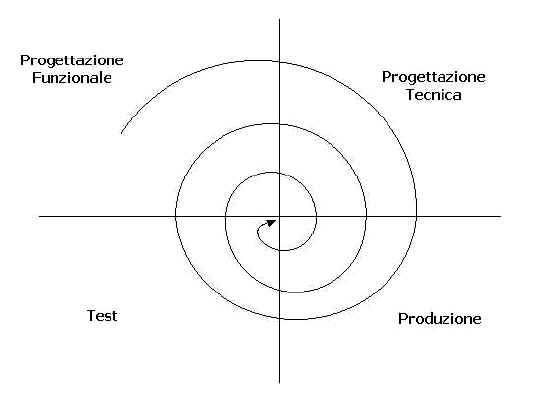
\includegraphics[width=.5\textwidth]{./capitoli/capitolo3/img/spirale}
\caption{Modello a spirale}

\end{figure}
\section{Pianificazione del Lavoro}


Per conseguire gli obiettivi di \textit{stage}, sono state preventivate circa 320 ore lavorative suddivise in 10 settimane durante l'arco temporale dal 17 Novembre 2014 al 30 Gennaio 2015, comprendente una pausa di una settimana per le vacanze natalizie. La suddivisione temporale effettuata a monte, assieme al responsabile interno ARPAV, è stata composta con una grana molto grossa, lasciandomi ampia libertà nell'organizzazione del lavoro a seconda delle mie necessità.

\begin{longtable}{ p{0.2\textwidth} | p{0.04\textwidth} | p{0.04\textwidth} | p{0.04\textwidth} | p{0.04\textwidth} | p{0.04\textwidth} | p{0.04\textwidth} | p{0.04\textwidth} | p{0.04\textwidth} | p{0.04\textwidth}  | p{0.04\textwidth}}
\textbf{Attività / \newline Settimana} & 1° & 2° & 3° & 4° & 5° & 6° & 7° & 8° & 9° & 10° \\
\endhead
\midrule
\textbf{\textit{{\color{OliveGreen}Analisi dei Requisiti}}} & 32 & 24  & / & / & / & / & / & / & / & / \\
\midrule
\textbf{\textit{{\color{OliveGreen}Progettazione Architetturale}}} & / & 8 & 32 & 20 & / & / & / & / & / & / \\
\midrule
\textbf{\textit{{\color{OliveGreen}Progettazione Dettagliata}}} & / & / & / & 12 & 25 & 10 & / & / & / & / \\
\midrule
\textbf{\textit{{\color{OliveGreen}Codifica}}} & / & / & / & / & / & 18 & 24 & 24 & 20 & 10 \\
\midrule
\textbf{\textit{{\color{OliveGreen}Testing}}} & / & / & / & / & 7 & 4 & 8 & 8 & 12 & 22 \\
\bottomrule
\caption{Suddivisione del lavoro}
\end{longtable}

Per ogni attività sono state preventivate le seguenti ore:

\begin{longtable}{ p{0.4\textwidth} | p{0.04\textwidth} }
\textbf{Attività} & \textbf{Ore}
\endhead
\midrule
\textit{Analisi dei Requisiti} & 56 \\
\midrule
\textit{Progettazione Architetturale} & 60 \\
\midrule
\textit{Progettazione Dettagliata} & 47\\
\midrule
\textit{Codifica} & 96 \\
\midrule
\textit{Testing} & 61 \\
\bottomrule
\caption{Ore per attività }
\end{longtable}

 
Nella figura (3.2) vengono evidenziate le suddivisioni temporali effettuate per lo svolgimento dello \textit{stage} e il susseguirsi delle attività. Le sezioni più chiare rappresentano i giorni non lavorativi del fine settimana, mentre le sezioni evidenziate di nero raffigurano le vacanze di Natale.
\begin{figure}[htbp]

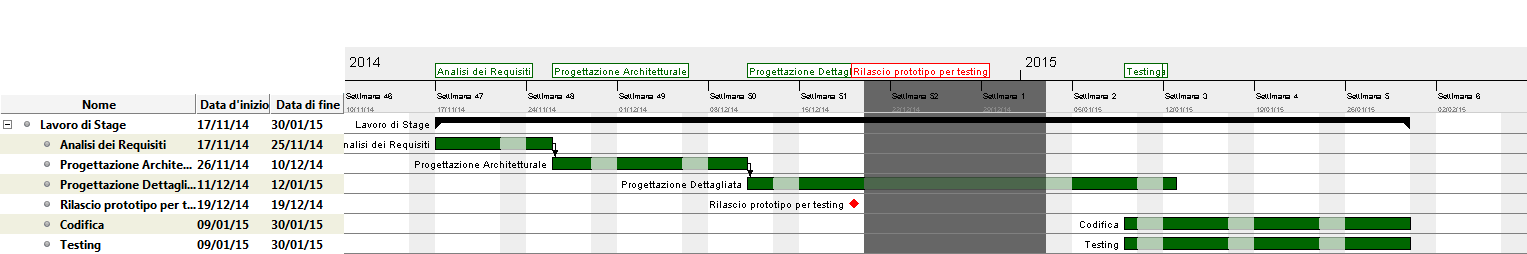
\includegraphics[width=1\textwidth]{./capitoli/capitolo3/img/da}
\caption{Diagramma di Gantt del periodo di Stage}
\end{figure}



\subsection{Preparazione al Lavoro di Stage}

In questa sezione illustro le modalità e gli esiti degli studi intrapresi per comprendere gli strumenti di lavoro. Le prime due settimane sono state suddivise in due sotto \textit{task}:

\begin{itemize}
\item \textbf{Studio del Dominio:} periodo dedicato all'acquisizione delle conoscenze di base delle tecnologie da utilizzare;
\item \textbf{Catalogazione dei Requisiti:} periodo dedicato allo studio dei requisiti e la catalogazione di quest'ultimi anche in relazione alle conoscenze appena acquisite.
\end{itemize}

\begin{figure}[htbp]	
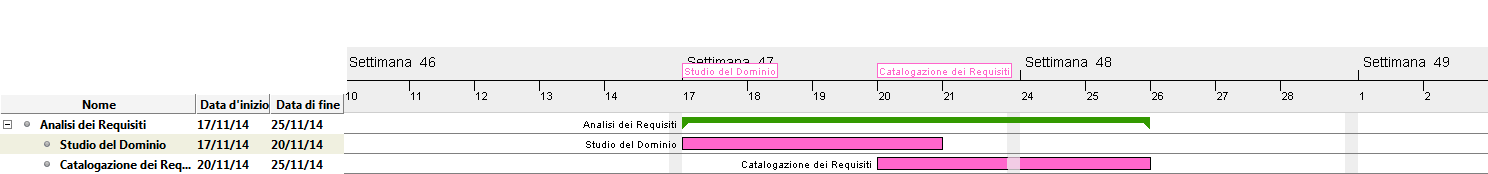
\includegraphics[width=1\textwidth]{./capitoli/capitolo3/img/requ}
\caption{Suddivisione lavoro prime due settimane}
\end{figure}





\subsubsection{Studio del Dominio}

L'universo Arduino si è affermato sul mercato ormai da diversi anni e ci sono molte tipologie di strumenti a supporto degli utenti neofiti e non. Prima dell'inizio dello \textit{stage} il responsabile del dipartimento di reti ed informatica mi ha dotato del manuale di base Arduino ( \textit{''Il Manuale di Arduino}'' Apogeo editore), grazie al quale ho potuto avvantaggiarmi acquisendo sufficienti conoscenze basilari che mi permettessero poi uno studio delle operazioni più complesse in sede di \textit{stage}. 

\begin{figure}[htbp]	
\centering
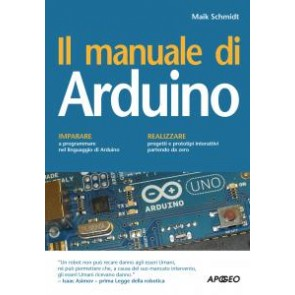
\includegraphics[scale=.5]{./capitoli/capitolo3/img/manuale}
\caption{Manuale Arduino}
\end{figure}

Entrato in possesso della strumentazione e dei dispositivi \textit{hardware} Arduino, mi sono affidato ai \textit{tutorial} presenti nel sito di Arduino (\url{http://www.arduino.cc/en/Guide/HomePage}) e degli esempi contenuti all'interno degli \textit{sketch} dell'IDE Arduino.
Per la ricerca delle librerie esterne da utilizzare durante lo sviluppo del progetto ho ricercato soluzioni appropriate nel sito Arduino, ma nel caso queste non fossero sufficienti o non adatte alle mie esigenze, ho effettuato ricerche più accurate utilizzando \textit{Google} come motore di ricerca.

Per la risoluzione di problemi, maggior parte delle volte, ho fatto uso del \textit{forum} dedicato (\url{http://forum.arduino.cc/}) nel quale moltissimi utenti, che hanno già avuto a che fare con problematiche simili, hanno illustrato soluzioni funzionanti. Nel caso queste non fossero sufficienti ho richiesto aiuto tramite \textit{mail} al responsabile del progetto del prototipo del pluviometro del FabLab di Verona.



\subsubsection{Studio delle Tecnologie}


\begin{itemize}



\item \textbf{Arduino UNO:}\\
Arduino UNO deve il suo nome perché trattasi della prima scheda rilasciata dalla casa. Le caratteristiche tecniche di questa scheda le permettono di supportare svariate tipologie di progetti con esigenze differenti. Per quanto riguarda il mio progetto, ciò che più miha  preoccupato era la limitata capacità di memoria interna al microcontrollore ATmega328 di 512Byte. I dati da memorizzare, i \textit{timestamp}, sono composti da più elementi:
\begin{itemize}
\item \textit{Data:} giorno/mese/anno;
\item \textit{Ora:} ore/minuti/secondi;
\item \textit{Contatore:} rappresentante il numero di \textit{timestamp} dall'ultima lettura.
\end{itemize}

Usando in totale 8 byte per ogni singolo \textit{timestamp} (3Byte per data, 3Byte per l'ora e 2Byte per il contatore), il numero massimo di \textit{timestamp} memorizzabili nella EEPROM del microcontrollore si limitano a 64. Ho così deciso di comprimere i dati per sfruttare al meglio la memoria, utilizzando 6 byte invece che 8:

\begin{longtable}{ p{0.2\textwidth} | p{0.2\textwidth} | p{0.2\textwidth} | p{0.2\textwidth}}
\textbf{Dato} & \textbf{Range valore} & \textbf{Non compresso} & \textbf{Compresso} \\
 \endhead
 \midrule
 \textit{Giorno} & 1-31 & 8bit & 5bit \\
 \midrule
 \textit{Mese} & 1-12 & 8bit & 4bit \\
 \midrule
 \textit{Anno} & 0-99 & 8bit & 7bit \\
 \midrule
 \textit{Ore} & 0-23 & 8bit & 5bit \\
 \midrule
 \textit{Minuti} & 0-59 & 8bit & 6bit \\
 \midrule
 \textit{Secondi} & 0-59 & 8bit & 6bit \\
 \midrule
 \textit{Contatore} & variabile\footnote{ : il contatore deve avere un \textit{range} di valori sufficientemente alto da non andare in \textit{overflow}. Inizialmente avevo valutato 16bit (0-65535), ma anche 15bit (0-32767) comprendono un insieme di numeri accettabile.} & 16bit & 15bit \\
 \midrule
 \textbf{Totale} & \textbf{-} & 64bit (8Byte) & 48bit (6Byte) \\
 \bottomrule
 \caption{Valori \textit{timestamp} compressione}
\end{longtable}

\begin{minipage}[c]{.5\textwidth}

\begin{longtable}{ p{0.18\textwidth} | p{0.05\textwidth}| p{0.05\textwidth}| p{0.05\textwidth}| p{0.05\textwidth}| p{0.05\textwidth}| p{0.05\textwidth}| p{0.05\textwidth}| p{0.05\textwidth}}
\textbf{Byte} & \multicolumn{7}{c}{\textbf{Composizione}} 
\endhead
\midrule
\textit{1° Byte} & m & m & m & g & g & g & g & g \\
\midrule
\textit{2° Byte} & a & a & a & a & a & a & a & m  \\
\midrule
\textit{3° Byte}  &  mi & mi & mi & o & o & o & o & o \\
\midrule
\textit{4° Byte}  &  s & s & s & s & s & mi & mi & mi  \\
\midrule
\textit{5° Byte}  &  c & c & c & c & c & c & c & s  \\
\midrule
\textit{6° Byte}  &  c & c & c & c & c & c & c & c  \\

\bottomrule
\caption{Conformazione \textit{bit timestamp}}
\end{longtable}
\end{minipage}
\hspace{10mm}%
\begin{minipage}[c]{.3\textwidth}

\begin{longtable}{ c{0.35\textwidth}  p{0.2\textwidth} }

\textbf{Simbolo} & \textbf{Valore}
\endhead

\textit{g} & Giorno \\

\textit{m} & Mese \\

\textit{a} & Anno \\

\textit{o} & Ore \\

\textit{mi} & Minuti \\

\textit{s} & Secondi \\

\textit{c} & Contatore \\

\end{longtable}

\end{minipage}


Utilizzando un algoritmo di compressione che porti la struttura di un \textit{timestamp} come descritto in tabella (3.4) si migliora la capacità della memoria da 64 \textit{timestamp} salvabili a 85, lasciando disponibili anche 2Byte per il salvataggio di dati supplementari. Ciononostante, effettuando una indagine iniziale, ho scoperto che durante una pioggia di forte intensità può verificarsi una basculata ogni due secondi. Utilizzando una memoria così limitata poco dopo 2 minuti si avrebbe un \textit{overflow} di memoria. Sottoposti questi dati al responsabile del dipartimento sono stati subito predisposti provvedimenti. Mi è stato proposto l'utilizzo di un \textit{microchip} di memoria supplementare nel quale salvare i \textit{timestamp} dalle capacità superiori.  

\item \textbf{C++}\\

\begin{figure}[htbp]
\centering

\includegraphics[width=0.15\textwidth]{./capitoli/capitolo3/img/c}
\caption{Logo C++}
\end{figure}

La scelta del linguaggio, C++, è stata una scelta importante per lo sviluppo del progetto. Le motivazioni che mi hanno spinto a scegliere questo linguaggio sono le seguenti:

\begin{itemize}
\item \textbf{Memoria Arduino UNO:} la scheda Arduino UNO possiede una \textit{memoria SRAM}\ped{g} di 2Kb appena. Utilizzare al meglio la poca memoria disponibile è assolutamente fondamentale;
\item \textbf{Riutilizzo del codice:} la quasi totalità del codice già presente \textit{online} e le librerie che supportano i moduli \textit{hardware} sono interamente scritti in C++;
\item \textbf{Conoscenza:} C++ è il linguaggio di programmazione con cui ho lavorato di più durante il mio percorso accademico.
\end{itemize}

Da queste motivazioni ne sono derivate delle conseguenze che mi hanno permesso una maggiore efficienza del progetto e una maggiore efficacia nella realizzazione:
\begin{itemize}
	\item \textbf{Memoria Arduino UNO:} con C++ la gestione della memoria viene delegata al programmatore, rendendo la programmazione più complicata, ma più efficace. Grazie a questo fattore del linguaggio è possibile sapere con certezza che la scheda non si bloccherà mai a causa dell'esaurimento della memoria SRAM;
	\item \textbf{Riutilizzo di codice:} la presenza di codice già pronto e funzionante velocizza la parte del lavoro di codifica;
	\item \textbf{Conoscenza:} la previa conoscenza del linguaggio mi permette di procedere con velocità durante la codifica e di usare le \textit{featuring} del linguaggio in modo efficiente ed efficace.
\end{itemize}   

\newpage

\item \textbf{EEPROM 24LC256}\\

\begin{figure}[htbp]
\centering
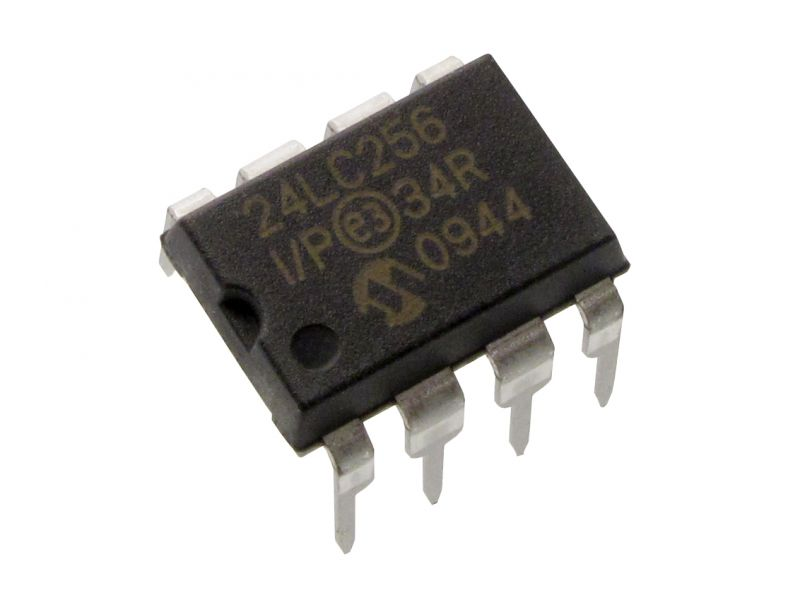
\includegraphics[width=.25\textwidth]{./capitoli/capitolo3/img/micro}
\caption{Microcip 24LC256}
\end{figure}

\textit{Hardware} scelto per compensare la bassa capacità di memoria di Arduino UNO. Questo componente, possedendo una capacità di 32Kb, colma il problema del salvataggio dei \textit{timestamp}, passando da 85 a 5461. 

E' possibile interfacciarsi con la memoria tramite la libreria \textit{Wire}.

\item \textbf{Protocollo I2C:}\\
E' stato richiesto come vincolo di progetto l'utilizzo del protocollo I2C per lo scambio di informazioni tra le componenti \textit{hardware}. Questo protocollo possiede ottime capacità di scambio di informazione a basso consumo a discapito di velocità, raggio d'azione e flessibilità. In Arduino il protocollo I2C è ampiamente supportato da una libreria interna denominata \textit{Wire}, nel cui sito (\url{http://www.arduino.cc/en/reference/Wire}) si possono trovare tutte le informazioni per il suo utilizzo.

Studiando a fondo le specifiche tecniche della libreria \textit{Wire} ho valutato che la banda di 32Byte per protocollo poteva essere un problema che limitasse la velocità di trasmissione dei dati. E' stato quindi necessario prendere in considerazione questo elemento come fattore di possibili problematiche.


\item \textbf{Tiny-RTC} \\
Il modulo \textit{hardware} in questione funziona sia come orologio, cioè ritornando data ed ora precisa in caso di richiesta, sia da \textit{sveglia} o \textit{allarme}. E' infatti possibile collegare il segnale di \textit{interrupt}  con la scheda Arduino e ricevere così una interruzione qualora l'ora preimpostata sia giunta. Oltre a ciò, la \textit{Tiny-RTC} non presenta ulteriori particolarità, se non il fatto che è predisposto dai produttori un protocollo tramite la libreria \textit{Wire} per l'interrogazione dell'\textit{hardware}.
\end{itemize}



\section{Analisi dei Requisiti}



\subsection{Classificazione dei Requisiti}

I requisiti sono stati suddivisi per ambito, tipologia e priorità:
\begin{itemize}
	
	\item \textbf{Ambito}
		\begin{itemize}
			\item \textit{Scheda Slave (S) :} requisito legato alla scheda Slave del progetto;
			\item \textit{Libreria Master (M) :} requisito legato alla libreria Master del progetto;
			\item \textit{Altro (A) :} requisito che esprime un ambito diverso dai precedenti.
		\end{itemize}
	\item Tipologia
		\begin{itemize}
			\item \textit{Funzionale (F) :} requisito che esprime una funzionalità del progetto;
			\item \textit{Vincolo (V) :} requisito che esprime un vincolo che il progetto deve soddisfare;
			\item \textit{Prestazionale (P):} requisito che esprime una condizione di \textit{performance} che il progetto deve soddisfare.
		\end{itemize}
		\item  \textbf{Priorità}
		\begin{itemize}
			\item \textit{Requisito Obbligatorio (O) :} requisito obbligatori ai fini del completamento dello \textit{stage};
			\item \textit{Requisito Desiderabile (D) :} requisito che fornisce valore aggiunto al progetto di \textit{stage}, ma che non rappresenta una condizione necessaria per la conclusione dei lavori.
		\end{itemize} 
\end{itemize}

\subsection{Individuazione dei Requisiti}

La maggior parte del materiale informativo, che mi ha permesso di compilare la lista dei requisiti, è stato acquisito durante le prime riunioni, precedenti l'inizio dei lavori, assieme al responsabile del dipartimento e il responsabile di FabLab.
Contemporaneamente allo studio del dominio, tenendo informati tramite \textit{mail} i responsabili dei progetti di FabLab e RaspiBO, ho identificato nuovi requisiti di progetto. 


\begin{longtable}{ p{0.18\textwidth} | p{0.62\textwidth }}

\textbf{Identificativo} & \textbf{Descrizione}
\endhead
 \midrule
\textit{SVO1} & Riconoscere gli \textit{interrupt} inviati dal pluviometro \\
 \midrule
\textit{SVO2} & Riconoscere segnali falsi positivi inviati dal pluviometro \\
 \midrule
\textit{SVO3} & Salvare i \textit{timestamp} in un formato compresso nel \textit{microchip} di memoria 24LC256 \\
 \midrule
\textit{SVO4} & Tener traccia dell'ultimo \textit{timestamp} letto dalla scheda Master \\
 \midrule
\textit{SVO5} & Interrogare tramite I2C la \textit{Tiny-RTC} per recuperare ora e data \\
 \midrule
\textit{SVO6} & Fornire un protocollo di interrogazione I2C per la scheda Master \\
 \midrule
\textit{SVO7} & Progettare il \textit{software} in modo da poter implementare nuovi protocolli di interfacciamento in  modo semplice \\
 \midrule
\textit{SPO8} & Inviare i \textit{timestamp} compressi tramite protocollo I2C per velocizzarne il processo del 20\% \\
 \midrule
\textit{SPO9} & Organizzare l'invio dei dati in modo da non riempire la memoria SRAM della scheda Slave o Master, senza superare quindi i 1200Kb\footnote{1200Kb sono un valore che si presta ad essere ottimale in una scheda Arduino UNO, in cui sono presenti 2Kb di memoria SRAM} \\
 \midrule
\textit{SPO10} & Organizzare la gestione della memoria secondo un algoritmo  \textit{round-robin} \\
 \midrule
\textit{SFO11} & Inviare i \textit{timestamp} tramite protocollo I2C non ancora letti alla scheda Master \\
 \midrule
\textit{SFO12} & Inviare i \textit{timestamp} presenti in memoria \\
 \midrule
\textit{SFO13} & Cancellare i \textit{timestamp} già letti, mantenendo quelli da leggere \\
 \midrule
\textit{SFO14} & Cancellare i \textit{timestamp} presenti in memoria e ripristinare al valore di \textit{default} i contatori \\
 \midrule
\\
 \midrule
\textit{MVO15} & Interrogare tramite I2C la scheda Slave \\
 \midrule
\textit{MVO16} & Progettare il \textit{software} della libreria in modo da poter implementare nuovi protocolli di interfacciamento in modo semplice \\
 \midrule
\textit{MFO17} & Richiedere i \textit{timestamp} non ancora letti \\
 \midrule
\textit{MFO18} & Richiedere i \textit{timestamp} presenti in memoria \\
 \midrule
\textit{MFO19} & Richiedere la cancellazione dei \textit{timestamp} già letti \\
 \midrule
\textit{MFO20} & Richiedere il ripristino della memoria \\
 \midrule
\textit{MFO21} & Convertire i dati da formato compresso in un formato semplice da utilizzare \\
 \midrule
\\
 \midrule
\textit{AVO22} & Fornire la documentazione \textit{online} della struttura \textit{software} e dei metodi del progetto \\
 \midrule
\\
 \midrule
\textit{SVD23} & Progettazione e realizzazione \textit{board} personalizzata con il codice funzionante della scheda Slave \\
 \midrule
\textit{MFD24} & Convertire i dati da formato compresso in JSon \\
 \midrule
\textit{AVD25} & Creare un \textit{software} per l'interfaccia con una scheda Master Arduino o Arietta \\
 \midrule
\textit{AVD26} & Creare una interfaccia \textit{web} per l'interazione con la scheda Master con Arietta \\
 \midrule
\textit{AVD27} & Trasportare il codice della scheda Slave da \textit{board} Arduino a \textit{board} Arietta \\
 \bottomrule

\caption{Requisiti}
	

\end{longtable}

\subsubsection{Strumenti Utilizzati}

Per il tracciamento dei requisiti sono stati utilizzati dei foglio \textit{online} di \textit{Google Drive}, i quali venivano aggiornati di volta in volta durante il periodo di tracciamento. Alla fine del processo di individuazione, i requisiti sono stati approvati dal responsabile interno ARPAV e dal responsabile del FabLab di Verona. Il ritardo nelle risposte del responsabile di RasbiBO non mi ha permesso di avere un suo riscontro iniziale nella trattazione dei requisiti.
\subsection{Casi d'Uso}

Trattandosi di un progetto in cui le relazioni sistema utente sono limitate, ho ritenuto non fosse necessario introdurre grafici di casi d'uso.  

\subsection{Dettagli Degni di Nota}

Durante la realizzazione avanzata del prodotto, RasbiBO mi ha richiesto di aggiungere un particolare requisito al sistema del progetto:

\begin{longtable}{ p{0.18\textwidth} | p{0.62\textwidth }}
\textit{SPO} & il sistema deve essere in grado di supportare richieste di lettura da parte della scheda Master ogni 5 secondi
\end{longtable}

Il seguente requisito è stato introdotto a progetto già in stato avanzato di lavoro. Questo tipo di richiesta vede pressoché inutile l'utilizzo di un dispositivo esterno di memoria, poiché ogni 5 secondi, al massimo, possono essere salvati circa 10 \textit{timestamp}. Poiché questi vengono letti in così poco tempo che mitigano il rischio di \textit{overflow}, a meno di interruzione delle comunicazioni. Dopo un'attenta valutazione durante una riunione con il dirigente interno di ARPAV, ho deciso che il carico di lavoro per soddisfare questo requisito non era tale da impedirmi di finire il mio lavoro in tempo. Ho dunque creato un \textit{fork} del progetto da dedicare per RasbiBO, in cui i \textit{timestamp} compressi vengono salvati all'interno della memoria EEPROM della scheda, mentre il \textit{branch} principale avrebbe seguito la normale tabella dei requisiti inizialmente accordata con FabLab di Verona.


\section{Progettazione e Codifica}

Definiti i limiti del progetto con l'approvazione dei requisiti, ho iniziato l'attività di progettazione. Prima di iniziare a la parte relativa le componenti \textit{software}, ho realizzato la struttura \textit{hardware} del progetto, in modo da avere la base su cui lavorare.



\subsection{Introduzione Architettura Hardware}

Le componenti \textit{hardware} sono state connesse fra di loro utilizzando una \textit{bread board}, una basetta di plastica che permette rapide connessioni fra strumenti \textit{hardware}. 

\begin{figure}[htbp]
\centering
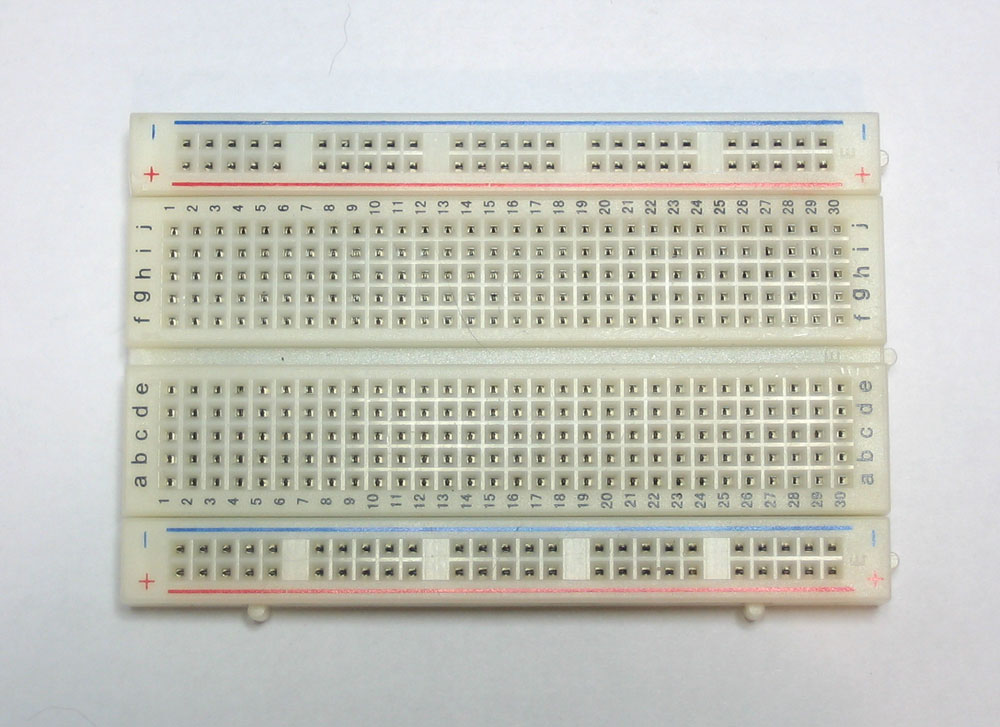
\includegraphics[width=.3\textwidth]{./capitoli/capitolo3/img/bread}
\caption{Scheda \textit{bread board}}
\end{figure}

L'utilizzo di questo strumento ha permesso durante il periodo di \textit{stage} un facile e veloce cambiamento delle connessioni delle componenti, facilitando la ricerca della struttura corretta.

\begin{figure}[htbp]
\centering
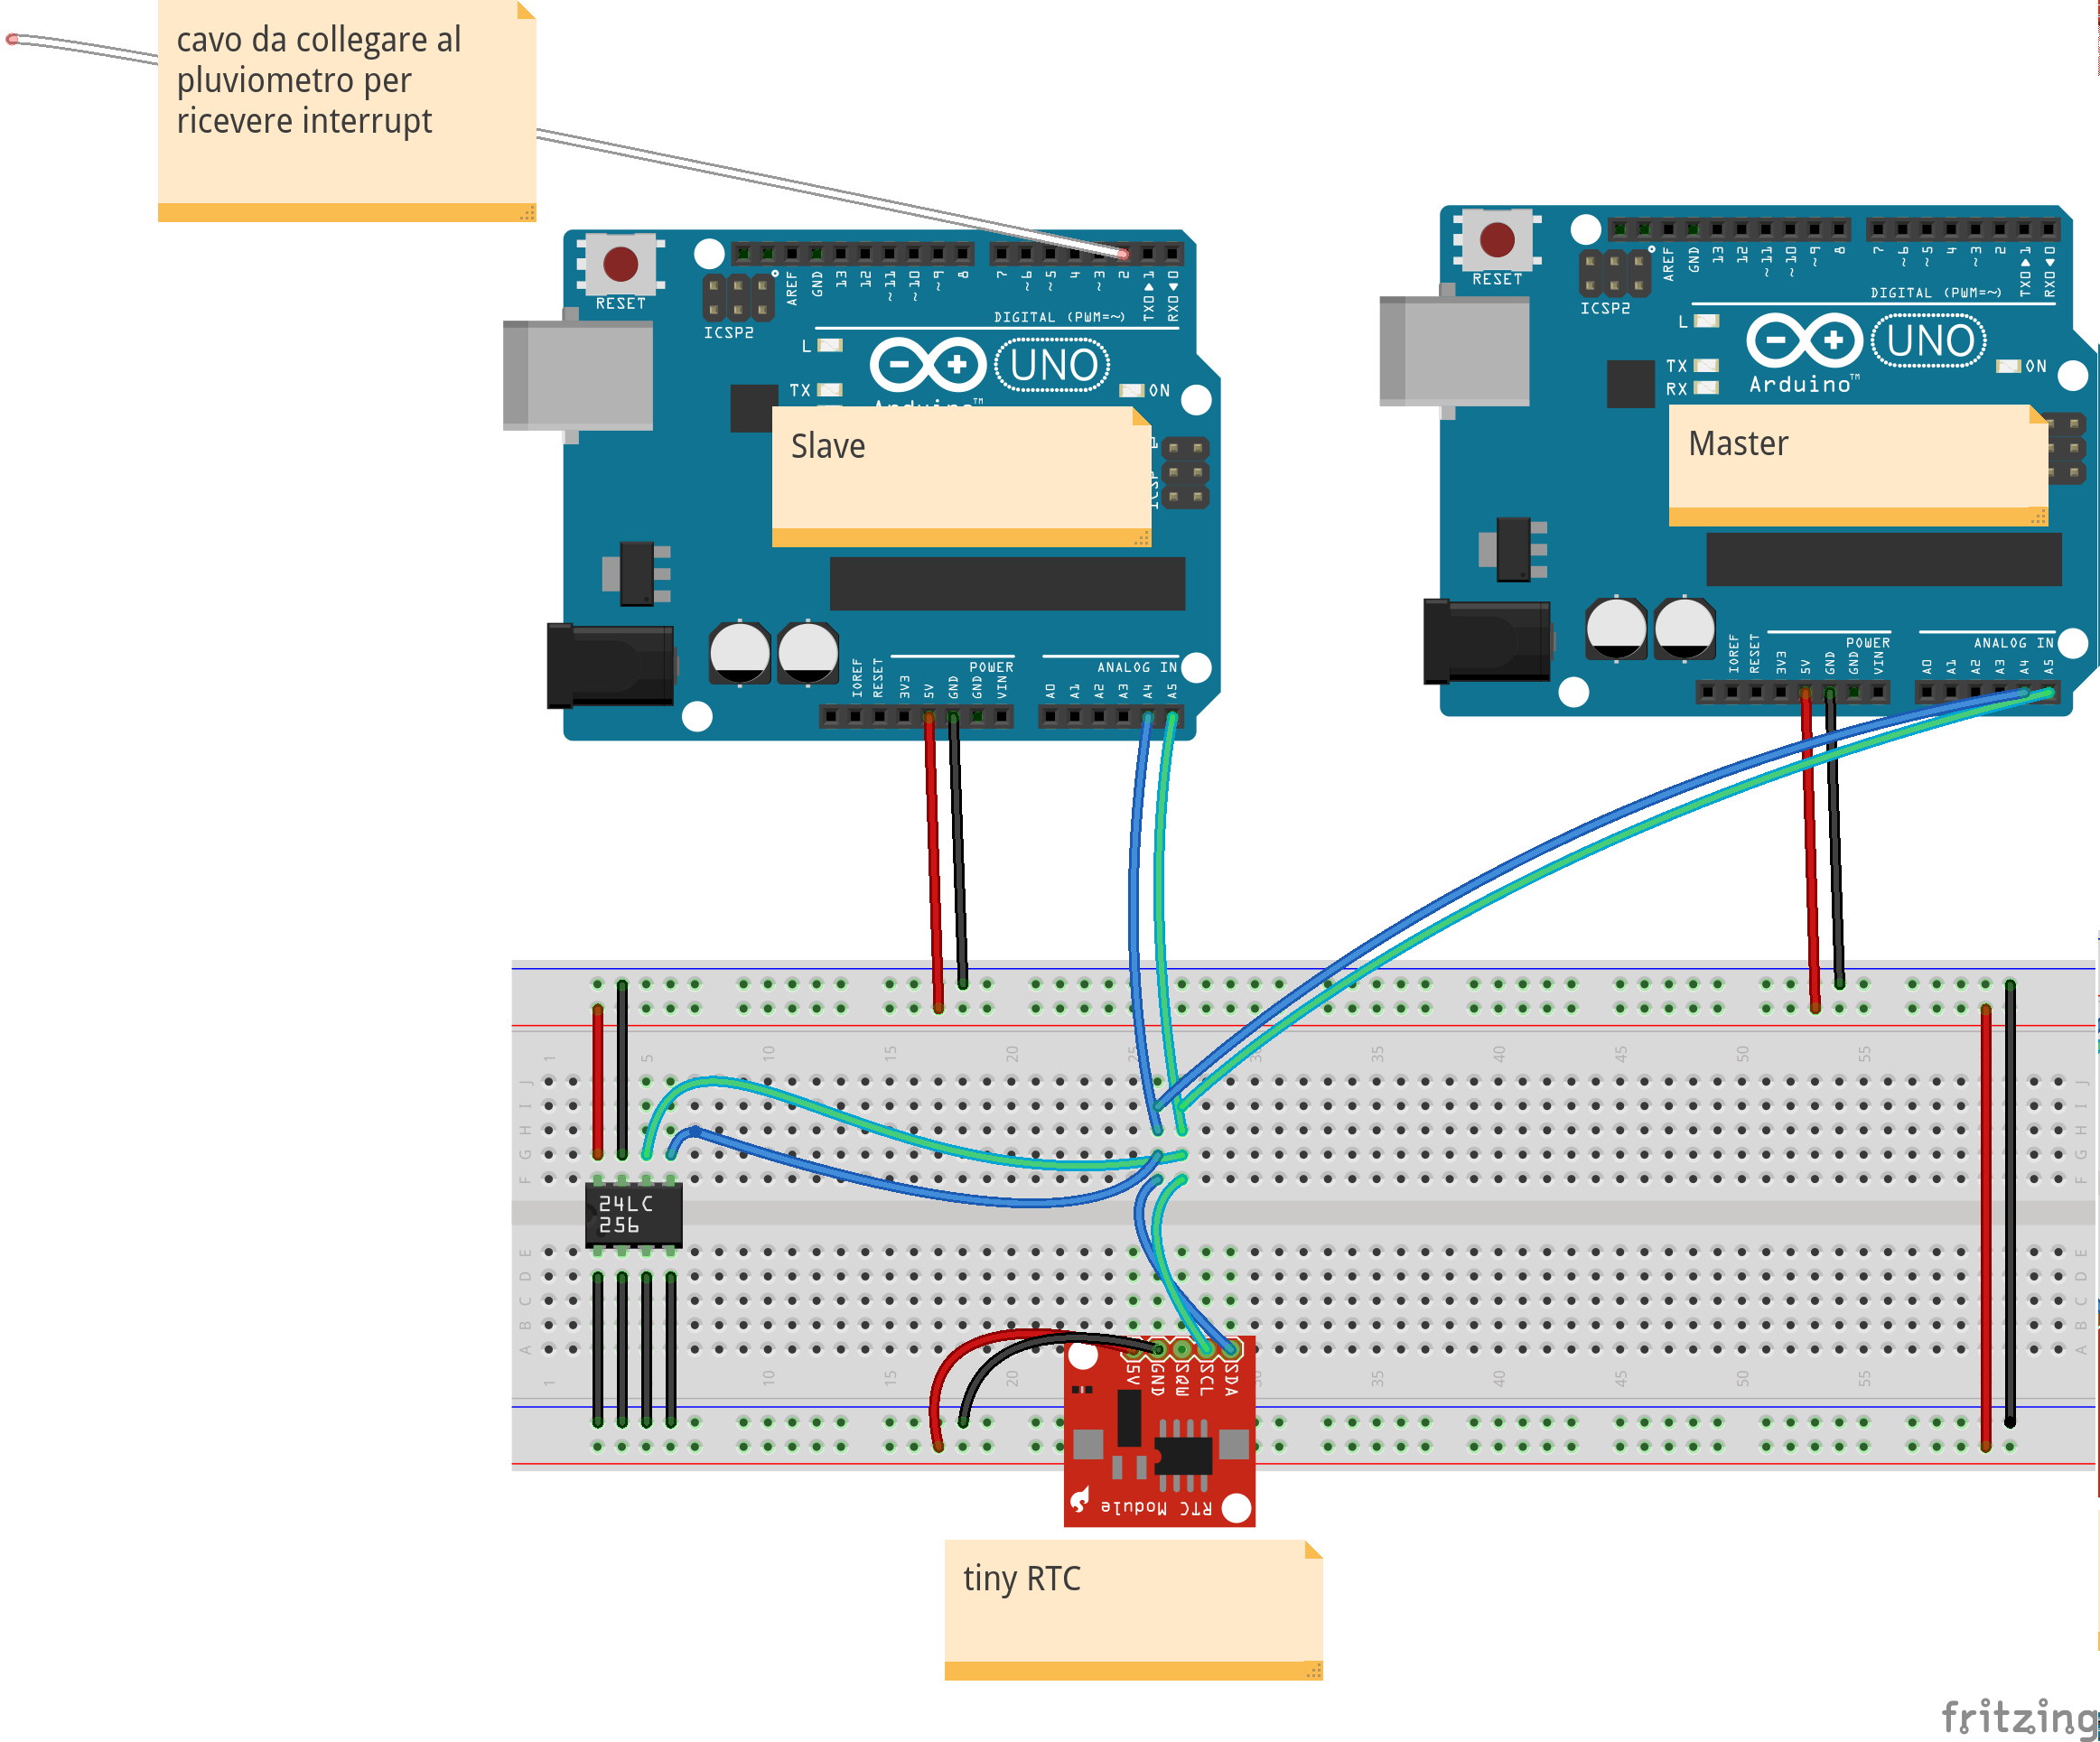
\includegraphics[width=.7\textwidth]{./capitoli/capitolo3/img/schema}
\caption{Schema elettronico progetto}
\end{figure}

Nella precedente figura (3.8) viene riportato lo schema elettronico delle connessioni delle componenti. Tramite l'utilizzo della \textit{bread board} è stato possibile simulare un \textit{bus} di comunicazione I2C, che mette in relazione tutte le componenti fra di loro. Successivamente con la realizzazione della \textit{board} Slave personalizzata, verrà creato un blocco unico che incorporerà il microcontrollore ATmega328, il microchip 24LC256 e la \textit{Tiny-RTC}, lasciando due entrate per la connessione I2C con una scheda Master esterna e un componente \textit{reed}\ped{g}\footnote{ la bascula del pluviometro è provvista di un magnete, che ad ogni basculata, oscilla davanti al \textit{reed} posto dentro la board personalizzata. Questo processo produrrà la chiusura del contatto e quindi la creazione di una interruzione (\textit{interrupt})} per la lettura degli eventi del pluviometro. 

\begin{figure}[htbp]
\begin{minipage}[c]{0.5\textwidth}
\centering\setlength{\captionmargin}{0pt}
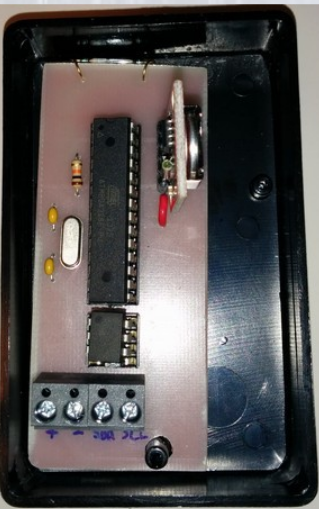
\includegraphics[width=.53\textwidth]{./capitoli/capitolo3/img/foto}
\caption{Foto prototipo \textit{board} personalizzata}
\end{minipage}
\hspace{10mm}%
\begin{minipage}[c]{0.5\textwidth}
\centering\setlength{\captionmargin}{0pt}
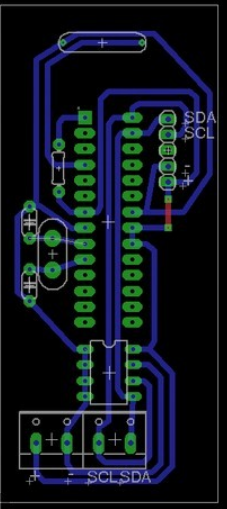
\includegraphics[width=.38\textwidth]{./capitoli/capitolo3/img/circuitoe}
\caption{Schema elettronico \textit{board} personalizzata}
\end{minipage}
\end{figure}

Verso la fine dei lavori durante la fase di \textit{testing} finale è stato utilizzata la \textit{board} personalizzata visibile in figura (3.9), con relativo schema elettronico in (3.10).
\subsection{Introduzione Architettura Software}

Le due componenti principali del sistema, scheda Slave e Master, devono dunque relazionarsi fra di loro tramite un protocollo prestabilito I2C, che consente lo scambio di informazioni qualora queste siano richieste. La libreria \textit{Wire} mette a disposizione delle funzioni che permettono la creazione di un sistema \textit{Slaves and Master} con Arduino. Stabilito l'indirizzo della scheda Slave\footnote{nel caso specifico è stato impostato l'indirizzo 2, ma può essere facilmente modificato dal codice sorgente, qualora questo indirizzo sia stato già inserito in un sistema \textit{Slaves and Master}}, la scheda Master invia un segnale nel bus I2C specificando che intende iniziare una comunicazione con 

\subsection{Architettura Libreria Scheda Master}

[:] Sezione in cui descrivo l'architettura della parte riguardante la libreria Master che permette di interfacciarsi con la Scheda Slave facilmente. 


\subsection{Architettura Scheda Slave}

[:] Sezione in cui descrivo l'architettura della Scheda Slave, che si interfaccia direttamente con il Pluviometro (questa parte è più ampia della precedente).

\subsection{Design Pattern Utilizzati}

[:] Sezione in cui elenco, motivo e descrivo i Design Pattern utilizzati nell'architettura del progetto.

\subsection{Dettagli Degni di Nota}

[:] Sezione in cui espongo alcuni dettagli rilevanti dell'architettura e soprattutto le difficoltà avute a causa delle limitate risorse hardware delle schede in mio possesso.

\subsection{Progettazione di Dettaglio e Codifica}

[:] Introduzione della sezione in cui spiego come mi sono adattato alle continue richieste di prototipi da parte dell'agenzia e come ho organizzato la progettazione in modo da rendere il codice facilmente modificabile e riutilizzabile per una codifica incrementale.

\subsubsection{Dettagli Degni di Nota}

[:] Sezione in cui descrivo alcuni metodi della libreria Master che permettono un facile interfacciamento con la scheda Slave. In aggiunta come sia possibile aggiungere facilmente nuove funzionalità al sistema senza alcuna iterazione, ma incrementando il codice.

\subsection{L'Utilizzo dei Prototipi}

[:] Breve sezione in cui spiego come, a causa delle necessità dell'ente, mi sia trovato costretto ad un continuo ciclo di "Progettazione, Codifica, \textit{test}, Progettazione Incrementale, Codifica, \textit{test}..", approccio diverso da quello affrontato durante il mio percorso accademico.

\section{Verifica e Validazione}

[:] Descrizione dell'attività di verifica e validazione e breve descrizione delle sottosezioni successive

\subsection{Analisi Statica}

[:] Elenco e descrizione degli strumenti utilizzati per l'analisi statica e alcuni valori che meritano d'esser presi in considerazione.

\subsection{\textit{test} sul Sistema Slave}

[:] Sezione in cui descrivo in dettagli i \textit{test} effettuati sulla scheda Slave, in progressione con gli incrementi effettuati.

\subsection{\textit{test} sul Sistema Master Slave}

[:] Descrizione dei \textit{test} effettuati sul sistema Slave integrato con le interazioni con la scheda master in progressione con gli incrementi effettuati.

\subsection{\textit{test} di Sistema}

[:] Descrizione dei \textit{test} effettuati sull'intero sistema.

\subsection{Dettagli Degni di Nota}

[:] Descrizione del problema degli impulsi "falsi positivi" inviati dal pluviometro, riscontrati durante i \textit{test} dell'intero sistema e soluzione.

\subsection{Consuntivo Orario Finale}

[:] Descrizione oggettiva e motivazione fra le discrepanze di orario preventivato ed effettivo in relazione agli obbiettivi raggiunti